
%%%%%%%%%%%%%%%%%%%%%%%%%%%
\chapter {Experimental Study on BVD in Arbitrary graph}
\label{Experiments}
%%%%%%%%%%%%%%%%%%%%%%%%%%%
 In this Chapter, we experimentally investigate the problem of black virus decontamination by studying the {\sc Castle-First} Strategy described in Chapter 6 and comparing it with the  {\sc Greedy} Exploration Algorithm \cite{cai}. 
The simulator we built is called {\sc ArbiBV}. We introduce its modeling methods and execution. The behavior, properties, and performance have been investigated through extensive computer simulation runs. The simulation results confirm the expected behavior/properties of the solution protocol.
%In particular, the result of the experiment has shown the following conclusion:
%\begin{enumerate}
%\item
%\item
%\end{enumerate}
%%%%%%%%%%%%%%%%%%%%%%%%%%%%%%%%%%%%%%%%%%%%%????????? ???
\section{The simulator}
\subsection{Simulation Model}
Our simulator only execute    the exploration phase, since the parameters (for example, the number of agents, the execution time \ldots) can be easily calculated after the location of the BV is detected (the time for the elimination phase is $O(1)$). In the simulator, we consider the worst possible scenario in terms of BV position, which actually corresponds to having no BV in the system, that is,   the agents have to explore the whole graph. The environment where the agents operate is a network modeled as a simple arbitrary undirected connected graph where each node has a unique ID (without loss of generality, from $1$ to $n$ where $n$ is the number of node in the graph). An agent is modeled as an entity with computational or information processing capability. All the agents follow the same protocol while their roles and the states can be different (for example, some of the agents are Leader Agents (LA) while some of the agents are Shadowing Agents (SA)). Note that our simulator does not have a Graphical User Interface(GUI). For monitoring purposes,  it provides a textual  description of the agents' activities only.   In each run of the simulator, we provide the number of nodes, the average degree of the graph, and the simulator generates an arbitrary graph based on that. After each run, the simulator calculates the number of agent deployed and the units of time elapsed.

\subsection{Simulation Sample graph} 
In this section, we compare the number of agents and the execution time between the {\sc Castle-First} Strategy and the sequential strategy of \cite{cai}, also between {\sc Castle-First} Strategy with different settings (sending different numbers of groups to explore the graph). When we compare our strategy with the sequential strategy.
We run our protocol in different graph settings; more precisely, network {\em size} $n$,  network {\em connectivity density} $NC$, and number of groups of agents deployed $m$, where the  connectivity density is defined as the ratio of the number of links of the graph with   the number of links in a complete graph with the same  number of nodes.
In our experiments we consider: $n=20,40,60,80,100$,     
$NC= 10\%, NC=20\%, \ldots, NC=100\% $, $m=1,2,3,4$. 

\color{blue} indicate what values of density are considered between $20 and 100\%$
\color{black}

For each specific setting (size of the graph,   network connectivity density,    number of groups of agents), we run the experiment for 50 times: the average execution time and the average number of agents needed would be the result of the execution time and the number of agents of this setting. So overall, we run 9020 experiments to obtain statistic data for our strategy.

By doing the comparison, we are interested in observing 
the time complexity of  our strategy   compared to the sequential one, and 
  the cost (in terms of additional agents) that we must pay for the faster speed.  

When we compare the results of different strategy settings of {\sc Castle-First} Strategy, we are interested in the following aspects: 
\begin{enumerate}
\item What is the relationship between the execution time and the number of agent groups that  participate in the strategy;
\item 
%Since in our strategy, given a certain group of agent group, we expect them to explore as many castles at the same time as possible (the advantage of distributed strategy would be more obvious), 
What is the impact of various topological factors (size,  connectivity, \ldots) on the efficiency of the strategy.
\end{enumerate}
%%%%%%%%%%%%%%%%%%%%%%%%%?????????????


\section{Simulation Results}
In this section, we compare the {\sc Castle-First} Strategy with the Sequential Strategy ({\sc Greedy} Exploration).
As a worst case scenario, we let the exploration proceed until all nodes are explored, without placing any black virus. 
For each network size, we create 10 connectivity levels and run our protocol with the number of groups ranging from one to four.

Simulation results show that the {\sc Castle-First} Strategy is never slower than the {\sc Greedy} Exploration, even when only one group of agents explores the graph,  and the extra cost in terms of the number of agents that we pay is acceptable. The time needed to finish the exploration of the graph in {\sc Greedy} Exploration and in the {\sc Castle-First} Strategy (where the number of exploring group ranging from one to four) is as shown in Figure \ref{fig:C_Move}

\begin{figure} [H] 
  \centering 
  \subfigure[size of graph:20 nodes ]{ 
    \label{fig:C_Move1:a} %% label for first subfigure 
    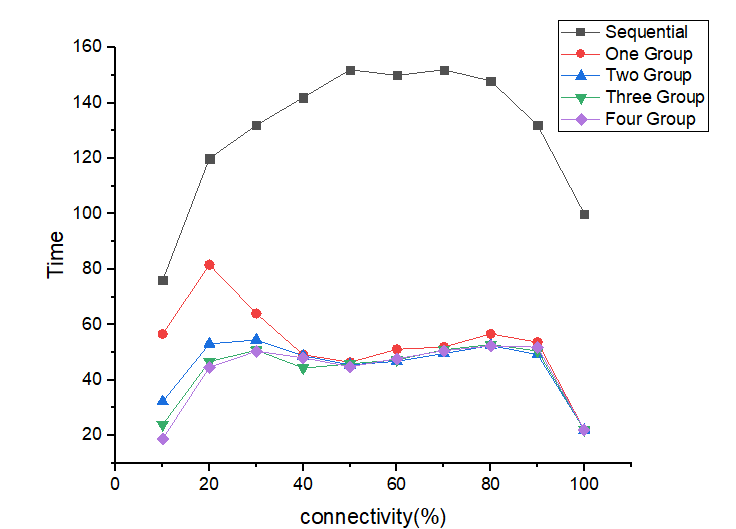
\includegraphics[width=2.2in]{figures/C_Move1.png}} 
%  \hspace{1in} 
  \subfigure[size of graph:40 nodes]{ 
    \label{fig:C_Move2:b} %% label for second subfigure 
    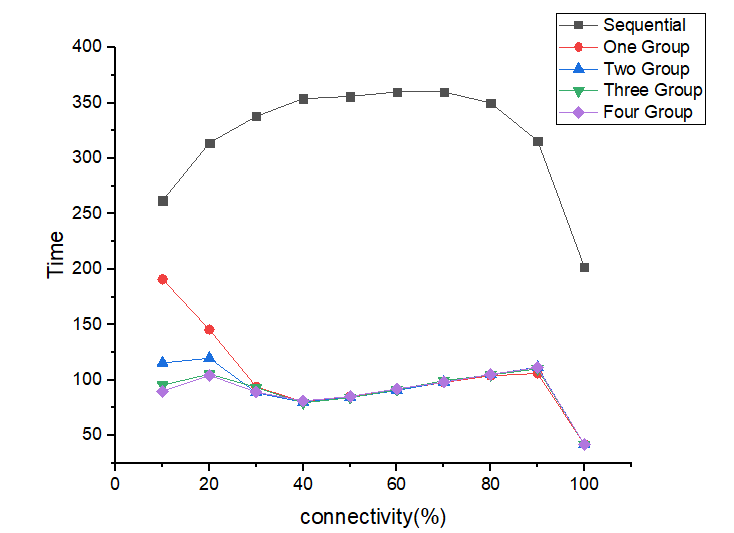
\includegraphics[width=2.2in]{figures/C_Move2.png}}
    \hspace{1in} 
  \subfigure[size of graph:60 nodes]{ 
    \label{fig:C_Move3:c} %% label for second subfigure 
    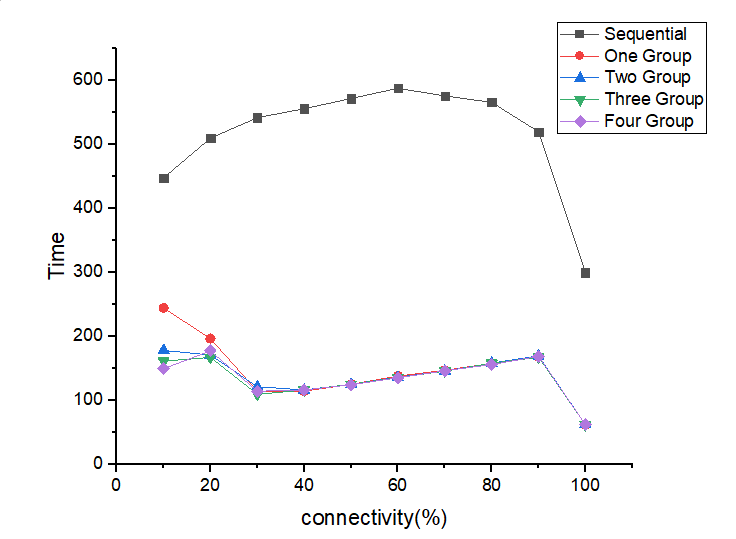
\includegraphics[width=2.2in]{figures/C_Move3.png}}
%      \hspace{1in} 
  \subfigure[size of graph:80 nodes]{ 
    \label{fig:C_Move4:d} %% label for second subfigure 
    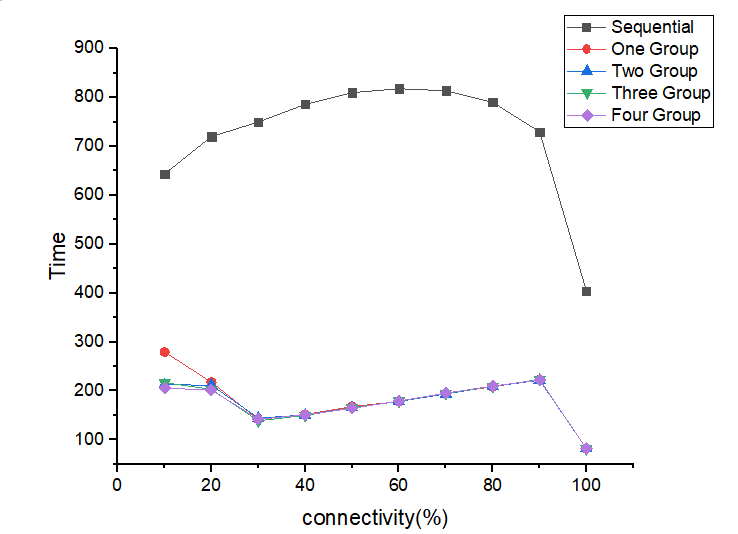
\includegraphics[width=2.2in]{figures/C_Move4.png}}
      \hspace{1in} 
  \subfigure[size of graph:100 nodes]{ 
    \label{fig:C_Move5:e} %% label for second subfigure 
    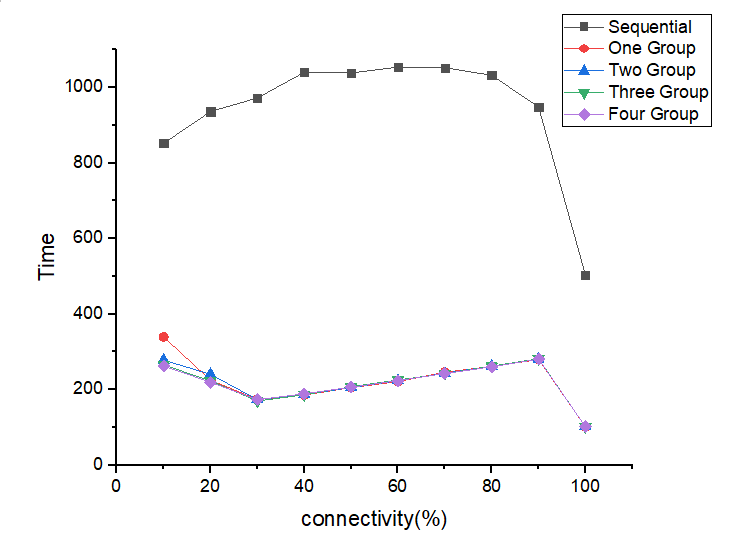
\includegraphics[width=2.2in]{figures/C_Move5.png}}
      \caption{Comparison between {\sc Greedy} Exploration and {\sc Castle-First} Strategy } 
  \label{fig:C_Move}%% label for entire figure 
\end{figure}

From Figure.\ref{fig:C_Move}, we have the following observations about the  time complexity:
\begin{enumerate}
\item \underline{Sequential Strategy ({\sc Greedy} Exploration) vs {\sc Castle-First} Strategy}: 

In all sizes of the graph, the time of the {\sc Greedy} Exploration increases gradually, reaching a maximum at 40\%-60\% connectivities, after that, it gradually decreases. It should be pointed out that the time costs are close for different graphs at 100\% connectivity level and are comparable or less than those at all 10\% connectivity level. While in the {\sc Castle-First} Strategy, the time cost first increases slightly and then decreases gradually to a minimum at 28\%-40\% connectivities, after that, it gradually increases to values comparable to those at all 10\%-20\% connectivities, and then decrease sharply to reach a minimum when the connectivity is 100\%. Note that,  though experiencing an increase from connectivity of 10 to 20 when the size of node is 20, the time increases less and less obviously as the size of the graph grows (an exception is the case of  ``one group" of agents, for  all sizes,  where  the time cost    always decreases   until it reaches a local minimum). When the size of the graph is 80, the time cost of the {\sc Castle-First} Strategy executed by more than one group stays at almost the same level from connectivity   10\% to 20\%. When the size of the graph is 100, the time directly decreases to the local minimum. This behavior is reasonable because,  as the size of the graph grows, even maintaining the same connectivity, the average degrees of nodes in the graph increase, which means the number of routes from one node to another increase to some extent, so when the agents move from one castle to another, they might have some shorter routes to choose, which saves time. The behavior of the ``one group" agent is largely influenced by this factor, so,  except in the graph of 20 nodes, the time cost with a single group does not experience a  slight increase but decreases directly to the local minimum.

After reaching the local minimum, the movement starts to increase. The reason is that, although there are shorter routes to choose as the connectivity increases when moving to the next castle (which saves time),  this advantage becomes less obvious because the length of the route from one node to another does not change significantly
 as the connectivity increases. At the same time, as the graph becomes denser, the castles are becoming larger, so we need to complete the ``Double Patrol" in large castles, which costs a significant amount of time. The result of the counteracting is that the movement increases after the local minimum movement. 

When the connectivity is larger than 90\%,  we observe the formation of a single very large castle.
%except for the home base,
% the combination of the other nodes becomes an extremely large castle so that in the exploration phase, the only thing we need to do is to explore one castle which results in the decrease of movement.
As a consequence,  in the exploration phase, the agents have to explore one castle, which results in a decrease of movement.  


\item \underline{  {\sc Castle-First} Strategy varying the number of  groups of agents.}

From   Figure \ref{fig:C_Move}, we can see that when the connectivity is larger than 30\%, the movements are almost the same no matter how many groups are sent to explore the graph. This can be explained; in fact,
  according to our algorithm, some of the castles in a graph have to be explored strictly sequentially (this is the case, for example, of some castles that are not accessible without first exploring others). 
This means that,  in some cases, even if there are castles unexplored and groups of agents available, full parallelism cannot be exploited.  In these situations,  sending more groups to explore the graph does not decrease time. So we prefer to use one group of agents executing the {\sc Castle-First} Strategy when the connectivity is larger than 20\%.

Another important observation is that as the size of the graph grows, the connectivity from where different group members perform similarly or almost the same is becoming smaller.


\end{enumerate} 

Based on the data presented in Figure \ref{fig:C_Move}, we now compare the time and the number of agents used by these two strategies. Since the time cost between the {\sc Castle-First} Strategy executed by different groups of agents is similar from connectivity 10\% to 100\% (especially when the connectivity is larger than 20\%),  we only compare the statistics between the {\sc Greedy} Exploration and the the {\sc Castle-First} Strategy with one group of agent. 
In figure \ref{fig:C_AT}, we show the ratio between the number of agents employed in the {\sc Castle-First} Strategy using a single group and the number of agents used in the {\sc Greedy} Exploration in the same situation.
We also show the ratio between the time incurred by the {\sc Castle-First} Strategy using one group of agents and the time incurred by the {\sc Greedy} Exploration.

\begin{figure} [H]
  \centering 
  \subfigure[Ratio between the number of agents used in {\sc Castle-First} with a single   group and  the number of agents used in {\sc Greedy}]{ 
    \label{fig:C_AT1:a} %% label for first subfigure 
    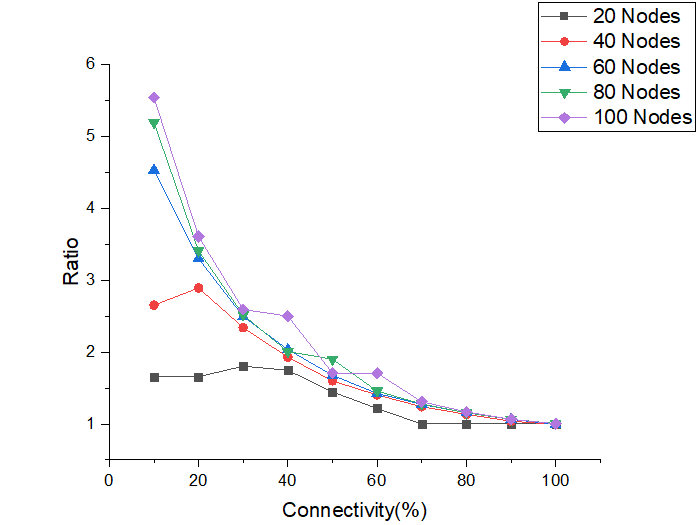
\includegraphics[width=2.5in]{figures/C_AT1.png}} 
    \hspace{1in} 
  \subfigure[Ratio between  time incurred by {\sc Castle-First}  using a single  group of agents
  and   time incurred by   {\sc Greedy}]{ 
    \label{fig:C_AT2:b} %% label for second subfigure 
    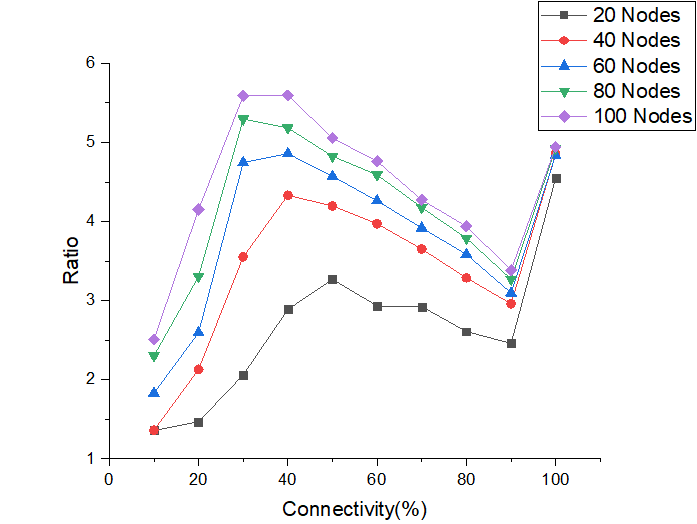
\includegraphics[width=2.5in]{figures/C_AT2.png}}
    \hspace{1in} 
    \caption{Ratio between   time and   agent cost of {\sc Castle-First}  using a single   group and 
     {\sc Greedy} in the same situation.} 
  \label{fig:C_AT} %% label for entire figure 
\end{figure}      
In Figure \ref{fig:C_AT}  (a)   the ratio is equal to number of agent used in the {\sc Castle-First} Strategy using a single group divided by the number of agents used in {\sc Greedy} Exploration 
(for convenience, we call it   ratio 1);    in Figure \ref{fig:C_AT}  (b), the ratio is equal to the time cost incurred by the  {\sc Castle-First} Strategy using a single group  divided by the time cost incurred by the {\sc Greedy} Exploration 
(for convenience, we call it  ratio 2).

From the Figure \ref{fig:C_AT}, we can make  the following observations:
\begin{enumerate}
\item As the connectivity grows, we can see that ratio 1 is decreasing, and when the connectivity is larger than 30\%, the ratio does not change a lot. When the connectivity is larger than 70\%, the ratio is near 1.
This tells us that when the connectivity is smaller than 20\%, we employ a much larger number of   agents (up to 5.5 times) than in the {\sc Greedy} Exploration,  while when the connectivity is between 30\% and  60\%, we use 1.2 to 2.5 times as many agents as that in the {\sc Greedy} Exploration. When the connectivity exceeds 70\%, we use almost the same number of agents as the ones used in the {\sc Greedy} Exploration.
\item Ratio 2 first increases reaching the local maximum when the connectivity reaches 30\% to 50\%, then decreases to the local minimum when the connectivity reaches 90\%; finally, it increases sharply to reach a maximum when the connectivity reaches 100\%.
\item Based on the two observations above, we come to the conclusion that, when the connectivity of the graph reaches 30\% to 50\%, the {\sc Castle-First} Strategy using a single group of agents works most efficiently.
\end{enumerate}

From the data we have shown in Figure \ref{fig:C_Move}   it appears that, except for the case of a single group,
the performances of different number of groups are similar,  even when the connectivity is only 10\%, so we compute the time cost at intervals of  10\% connectivity. 
To provide more precise statistics describing 
the behavior between 0 and   10\% connectivity (the connectivity from which the performance of different group numbers is similar or almost the same) we should look in more details at this interval.
% is smaller (including the performance of one group). 
%That is, we would like to focus on graphs with small connectivity.
It is obvious that for different graph sizes, even with the same connectivity, the degrees of the nodes are different so we  will use the   ``Average Degree"   to see if the results of the {\sc Castle-First} Strategy executed by different number of groups of agents have large difference depending on the average degrees of their nodes. The average degree of a graph is an important factor because it influences how the castles of the graph form. From the conclusion of Figure \ref{fig:C_Move}, we know that when the connectivity is larger than 10\% to 20\%, there are no big differences between   the time incurred by different groups of agents, so now we would like to start from a small degree of 2.5 and increase by 0.5  at each  time (as shown in Figure \ref{fig:Final})

\begin{figure} [H]
  \centering 
  \subfigure[size of graph:50 nodes]{ 
    \label{fig:Final1:a} %% label for first subfigure 
    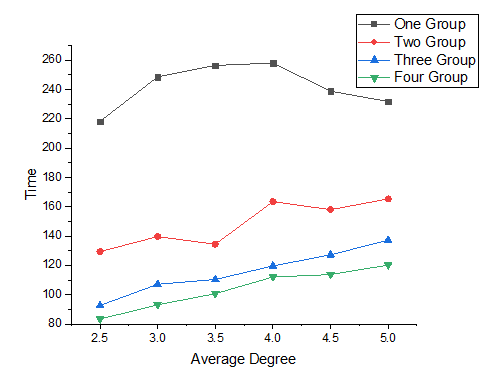
\includegraphics[width=2.5in]{figures/50.png}} 
    \hspace{1in} 
  \subfigure[size of graph:100 nodes]{ 
    \label{fig:Final2:b} %% label for second subfigure 
    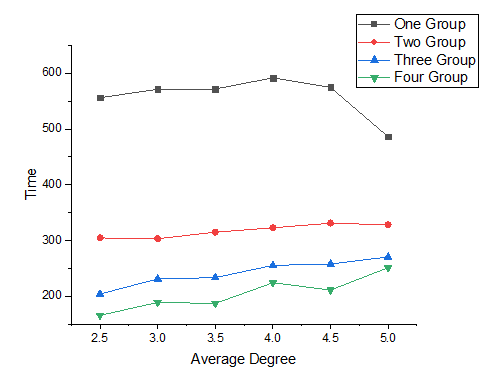
\includegraphics[width=2.5in]{figures/100.png}}
    \hspace{1in} 
      \subfigure[size of graph:150 nodes]{ 
    \label{fig:Final3:c} %% label for first subfigure 
    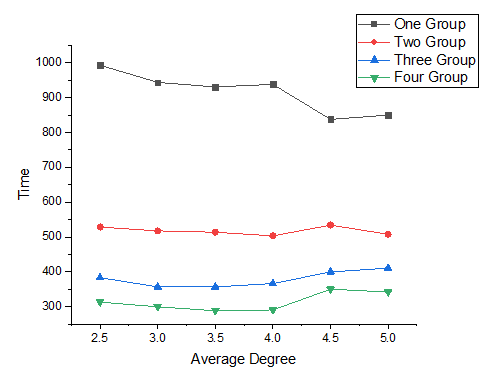
\includegraphics[width=2.5in]{figures/150.png}} 
    \hspace{1in} 
  \subfigure[size of graph:200 nodes]{ 
    \label{fig:Final4:d} %% label for second subfigure 
    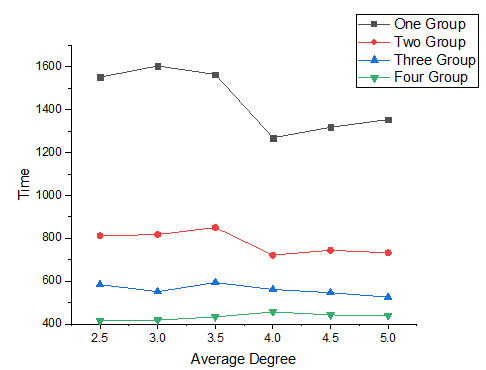
\includegraphics[width=2.5in]{figures/200.png}}
    \hspace{1in} 
      \subfigure[size of graph:250 nodes]{ 
    \label{fig:Final5:e} %% label for first subfigure 
    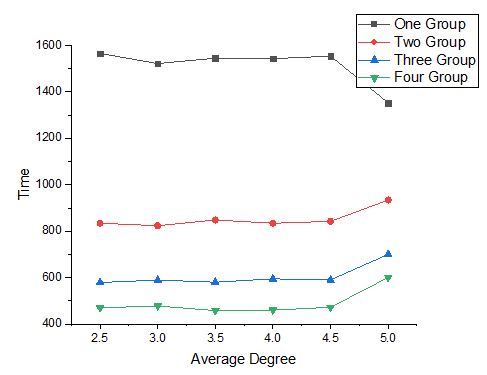
\includegraphics[width=2.5in]{figures/250.png}} 
    \hspace{1in} 
  \subfigure[size of graph:300 nodes]{ 
    \label{fig:Final6:f} %% label for second subfigure 
    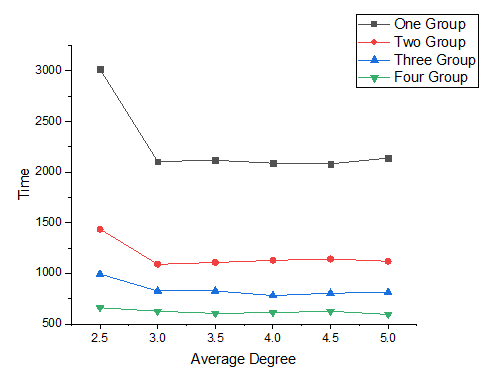
\includegraphics[width=2.5in]{figures/300.png}}
    \hspace{1in} 
    \caption{Time cost by different number of group} 
  \label{fig:Final} %% label for entire figure 
\end{figure}  

From the data obtained, we can make the following observations:
% ( for convenience, we call ``optimal average degree", the average degree where the difference between the time incurred by different numbers of groups is large (at least 100 unit of time)).   \color{blue} not clear what you mean: also, find another name, we cannot use optimal average degree ... \color{black}
 
\begin{enumerate}
\item For different group sizes, the largest difference in time cost can be observed between the strategy executed by one group and two groups of agents  (although there are still some decreases when we increase the number of groups executing the strategy, they are much smaller). Also, the difference in time cost when employing different group numbers is smaller as the average degree grows.

\item Excluding now the case of a single group, let us focus on the performance of other group numbers. When the size of the graph is 50, we can see that the performances of different group numbers are similar at the beginning (the difference between them is smaller than 50). When the size increases to 100, the difference   between different group members is more evident, and appears at the average degree of 2.5. What should be pointed out is that such a big difference exists between the time cost by two groups and three groups of agents. So, if we want to execute the strategy and decrease time when the size of the graph is smaller than 100 nodes, at most two groups of agents are recommended.

We also run experiments on larger  graphs  (when the number of nodes is bigger than 100). 
First note that, according to our conclusion based on Figure \ref{fig:C_Move}, as the size of the graph grows, the connectivities from where different group members perform similarly  become smaller. 
As a result, the average degree from where different group members perform similarly   increases, but very slowly. That is, like in the case of   small size graphs, the performance of different number of groups in larger graphs is still similar   when the average degree is larger than a certain number (this number might increase as the size of the graph grows,  but the increase is slow). From Figure \ref{fig:C_Move} (c) to (f), we can see that there are large differences between time cost by different group numbers (even between the time cost by three groups or even four groups of agent). When the size of the graph is 250 or 300, we can see that there are still  big differences between the performance of three groups and four groups of agents at an average degree of 5.0 (which is the maximum average degree shown in Figure \ref{fig:Final} )
We can see that at this interval (average degree from 2.5 to 5.0), as the size of the graph grows, the advantage of using more groups of agents is becoming more obvious, and this interval is longer as the size of the graph becoming larger.
 \end{enumerate}
%We can see that Though the difference of performance of different group numbers shows a  tendency to be similar when the average degree is larger than 5 (which is the maximum average degree shown in Figure \ref{fig:Final}  \color {blue} ??? from where we do not give the statistics, 

\section{Summary}
In this chapter, the parallel BVD problem in Castle-First Strategy is investigated experimentally. A large number of simulations on different size of graphs with many connectivity densities are carried out. The Castle-First Strategy beats the sequential strategy for all graph at each connectivity level even employing only one group of agent. Also, from the results, we have the following conclusions:
\begin{enumerate}
\item When the connectivity of the graph is larger than $20\%$, we prefer to use one group of agents executing the Castle-First Strategy because when the graph becomes denser, sending more groups to explore the graph does not decrease time.
\item When the connectivity of the graph reaches 30\% to 50\%, the Castle-First Strategy using a single group of agents works most efficiently: it is much faster than the sequential strategy and at the same time it employs similar number of agents to the sequential strategy.
\item At the interval of average degree from 2.5 to 5.0, as the size of the graph grows, the advantage of using more groups of agents is becoming more obvious (the time still experiences large decrease when employing more groups of agents to explore the graph) and this interval is longer as the size of the graph becoming larger.
\end{enumerate}















